\documentclass[a4paper,12pt]{extarticle}
\usepackage[utf8x]{inputenc}
\usepackage[T1,T2A]{fontenc}
\usepackage[russian]{babel}
\usepackage[hidelinks]{hyperref}
\usepackage{indentfirst}
\usepackage{listings}
\usepackage{color}
\usepackage{here}
\usepackage{array}
\usepackage{multirow}
\usepackage{graphicx}
\usepackage{subcaption} 
\usepackage{mathtools}
\usepackage{listings}

\usepackage{caption}
\renewcommand{\lstlistingname}{Программа} % заголовок листингов кода

\bibliographystyle{ugost2008ls}

\usepackage{listings}
\lstset{ %
extendedchars=\true,
keepspaces=true,
language=C,						% choose the language of the code
basicstyle=\footnotesize,		% the size of the fonts that are used for the code
numbers=left,					% where to put the line-numbers
numberstyle=\footnotesize,		% the size of the fonts that are used for the line-numbers
stepnumber=1,					% the step between two line-numbers. If it is 1 each line will be numbered
numbersep=5pt,					% how far the line-numbers are from the code
backgroundcolor=\color{white},	% choose the background color. You must add \usepackage{color}
showspaces=false				% show spaces adding particular underscores
showstringspaces=false,			% underline spaces within strings
showtabs=false,					% show tabs within strings adding particular underscores
frame=single,           		% adds a frame around the code
tabsize=2,						% sets default tabsize to 2 spaces
captionpos=t,					% sets the caption-position to top
breaklines=true,				% sets automatic line breaking
breakatwhitespace=false,		% sets if automatic breaks should only happen at whitespace
escapeinside={\%*}{*)},			% if you want to add a comment within your code
postbreak=\raisebox{0ex}[0ex][0ex]{\ensuremath{\color{red}\hookrightarrow\space}},
texcl=true,
inputpath=listings,                     % директория с листингами
}

\usepackage[left=2cm,right=2cm,
top=2cm,bottom=2cm,bindingoffset=0cm]{geometry}

%% Нумерация картинок по секциям
\usepackage{chngcntr}
\counterwithin{figure}{section}
\counterwithin{table}{section}

%%Точки нумерации заголовков
\usepackage{titlesec}
\titlelabel{\thetitle.\quad}
\usepackage[dotinlabels]{titletoc}

%% Оформления подписи рисунка
\addto\captionsrussian{\renewcommand{\figurename}{Рисунок}}
\captionsetup[figure]{labelsep = period}

%% Подпись таблицы
%\DeclareCaptionFormat{hfillstart}{\hfill#1#2#3\par}
%\captionsetup[table]{format=hfillstart,labelsep=newline,justification=centering,skip=-10pt,textfont=bf}

%% Путь к каталогу с рисунками
\graphicspath{{fig/}}

%% Внесение titlepage в учёт счётчика страниц
\makeatletter
\renewenvironment{titlepage} {
 \thispagestyle{empty}
}
\makeatother

\DeclarePairedDelimiter\abs{\lvert}{\rvert}%
\DeclarePairedDelimiter\norm{\lVert}{\rVert}%

\usepackage{amsmath}

\lstset{language=Java} 

\begin{document}	% начало документа

% Титульная страница
\begin{titlepage}	% начало титульной страницы

	\begin{center}		% выравнивание по центру

		\large Санкт-Петербургский политехнический университет Петра Великого\\
		\large Институт прикладной математики и механики \\
		\large Высшая школа прикладной математики и вычислительно физики \\[6cm]
		% название института, затем отступ 6см
		
		\huge Вычислительные комплексы\\[0.5cm] % название работы, затем отступ 0,5см
		\large \textbf{Курсовой проект}\\[5.1cm]

	\end{center}


	\begin{flushright} % выравнивание по правому краю
		\begin{minipage}{0.25\textwidth} % врезка в половину ширины текста
			\begin{flushleft} % выровнять её содержимое по левому краю

				\large\textbf{Работу выполнил:}\\
				\large Колесник Виктор\\
				\large {Группа:} 3630102/70201\\
				
				\large \textbf{Преподаватель:}\\
				\large к.ф.-м.н., доцент\\
				\large Баженов Александр Николаевич

			\end{flushleft}
		\end{minipage}
	\end{flushright}
	
	\vfill % заполнить всё доступное ниже пространство

	\begin{center}
	\large Санкт-Петербург\\
	\large \the\year % вывести дату
	\end{center} % закончить выравнивание по центру

\end{titlepage} % конец титульной страницы

\vfill % заполнить всё доступное ниже пространство


% Содержание
\renewcommand\contentsname{\centerline{Содержание}}
\tableofcontents
\newpage


\section{Постановка задачи}

Для демонстрации интервальной глобальной оптимизации использовать функцию:
\begin{equation}
	function [Z, Worklist] = globopt0(X).
\end{equation}
Она возвращает значение глобального экстремума $Z$ и рабочий список $WorkList$. Работа алгоритма построена на последовательном сужении множества, на котором ищется оптимум.

\subsection{Задача 1}

Рассмотреть пример из лекционного материала. Построить рабочий список, построить график сужения интервала.

\subsection{Задача 2}

Взять пример с сайта тестовых функций. Изучить сходимость метода.



\section{Теория}

\subsection{Алгоритм для глобальной минимизации функции}

Алгоритм $GlobOpt$ оперирует с рабочим списком $\mathcal{L}$, в котором будут храниться все брусы, получающиеся в результате дробления исходного бруса области определения на более мелкие подбрусы. Одновременно с самими подбрусами будем хранить в рабочем списке и нижние оценки областей значений целевой функции по этим подбрусам, так что элементами списка $\mathcal{L}$ будут записи-пары вида
\begin{equation}
	\mathcal{L}: (Y, y), where Y \subseteq X, y = f(Y)
\end{equation}

\subsection{Функция Растригина}

\begin{equation}
	f(x,y) = x^2 + y^2 - cos(18 * x) - cos(18 * y)
\end{equation}

Минимум функции достигается при значении аргумента $(x,y)=(0,0)$ и равен $-2$.

\newpage

\begin{figure}[h]
	\centering
	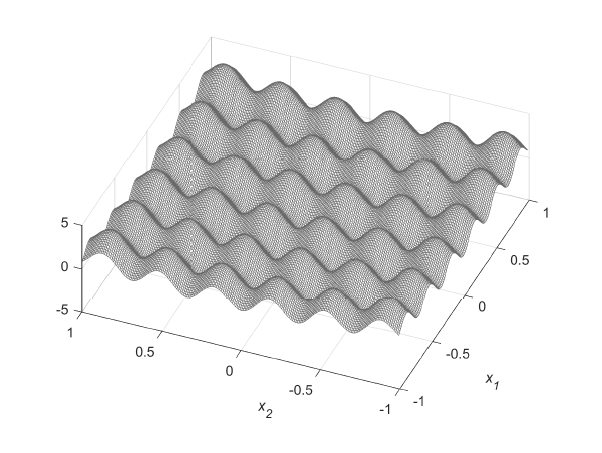
\includegraphics[width=0.75\textwidth]{rastrigin_plot.png}
	\caption{График функции Растригина}
\end{figure}

\subsection{Функция МакКормика}

\begin{equation}
	f(x,y) = sin(x + y) + (x - y)^2 - 1.5 * x + 2.5 * y + 1
\end{equation}

Минимум функции достигается при значении аргумента $(x,y)=(-0.54719,-1.54719)$ и равен $-1.9133$.

\newpage

\begin{figure}[h]
	\centering
	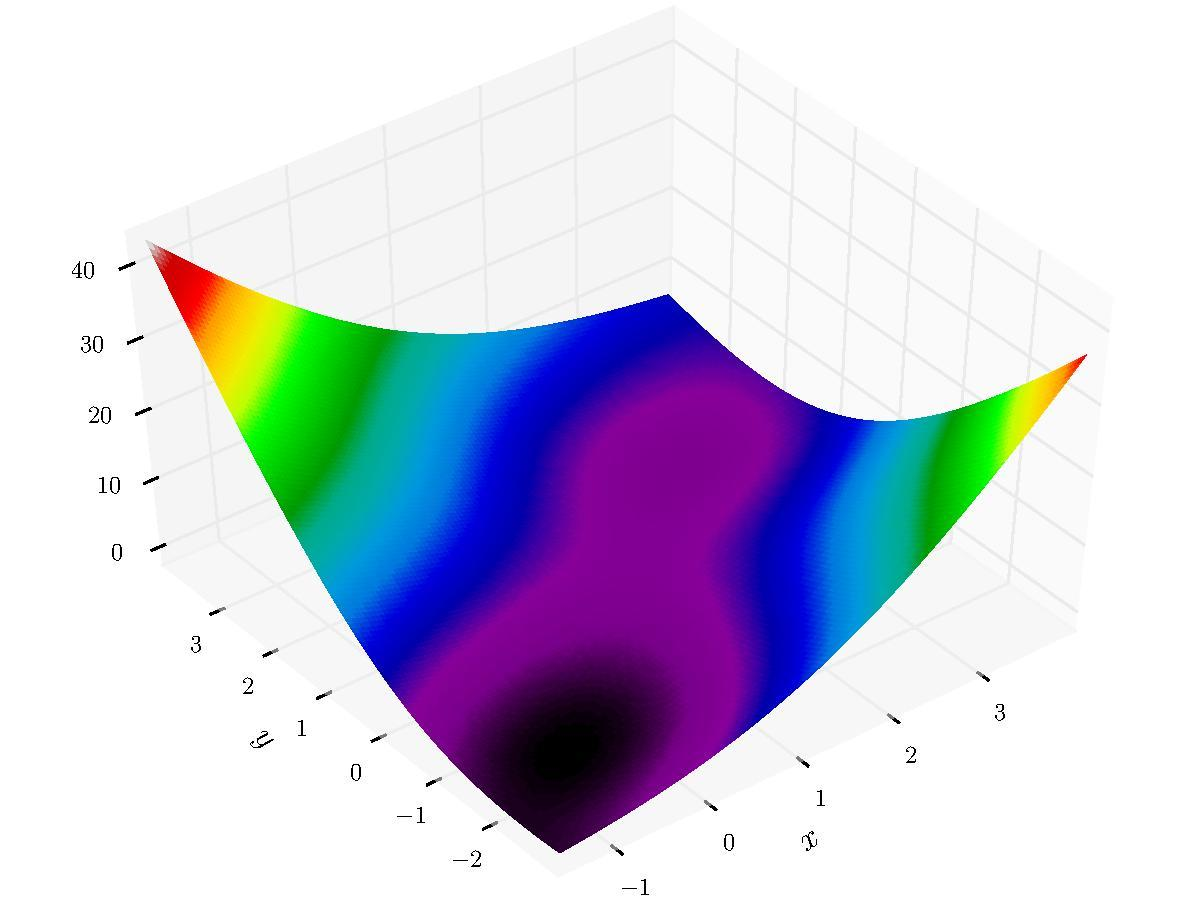
\includegraphics[width=0.75\textwidth]{mccormick_plot.jpg}
	\caption{График функции МакКормика}
\end{figure}



\section{Результаты}

\subsection{Задача 1}

Добавим в реализацию функции поиска глобального минимума сохранение ширины ведущего блока для каждого шага итерации в отдельный массив $widths$.  \\

Зададим максимальное количество итераций равным 200. \\

Начальное множество допустимых значений имеет вид: $X = [-5, 5] \times [-5, 5]$. \\

Полученное значение глобального экстремума $Z=-2$. \\

Последовательность значений ширины ведущего бруска представим в виде графика зависимости этой ширины от номера итерации. \\

\newpage

\begin{figure}[h]
	\centering
	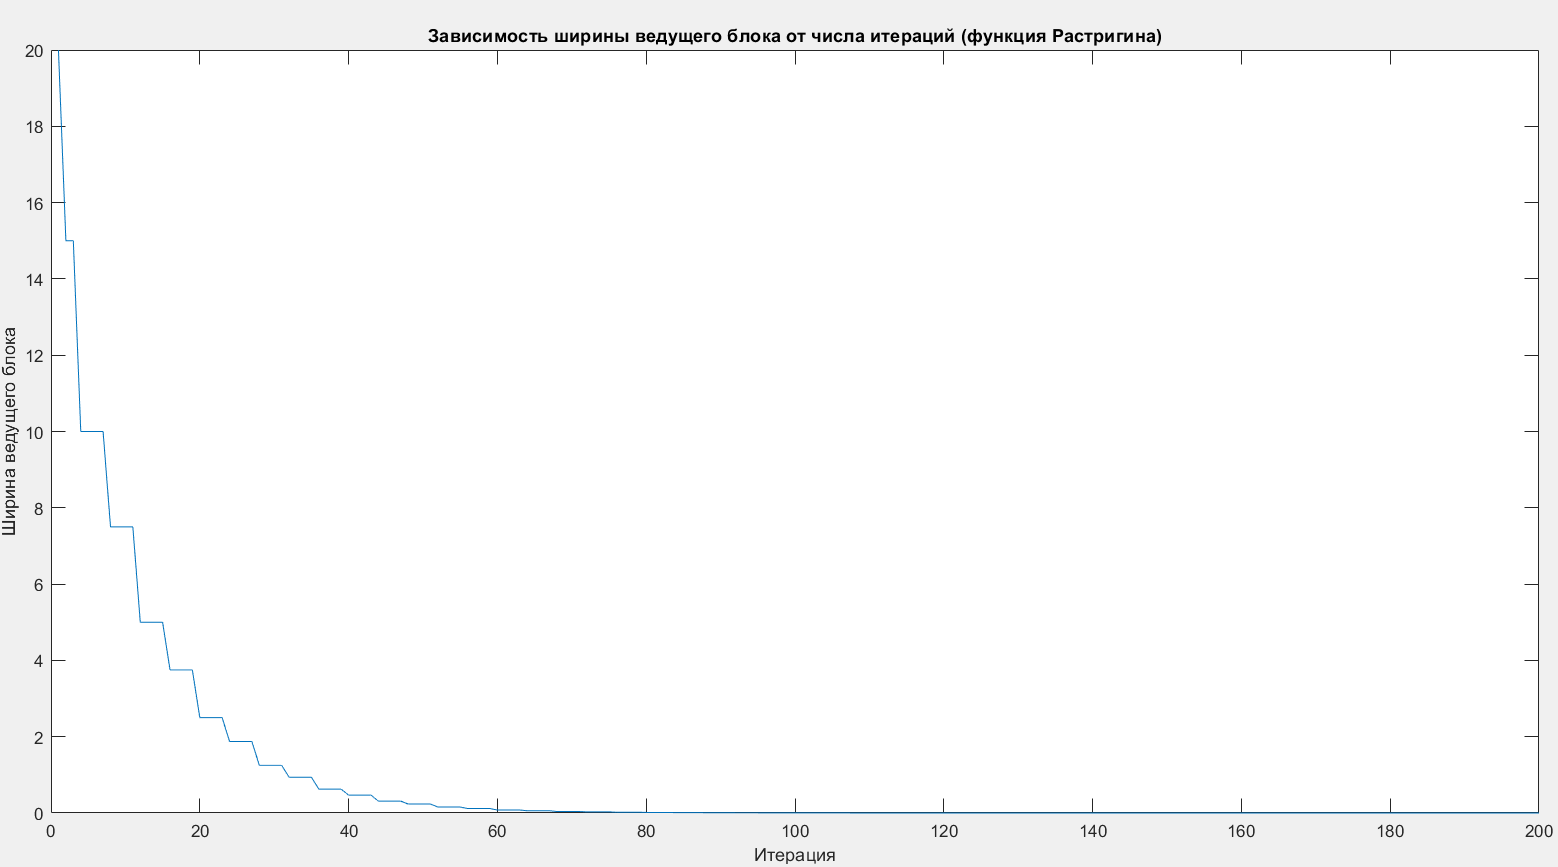
\includegraphics[width=0.75\textwidth]{rastrigin_width.png}
	\caption{Зависимость ширины бруска для функции Растригина}
\end{figure}

\subsection{Задача 2}

Начальное множество допустимых значений имеет вид: $X = [-1.5, 4] \times [-3, 4]$. \\

Посмотрим, как зависит полученный алгоритмом экстремум от количества итераций. Результаты представлены в таблице:

\begin{center}
	\begin{tabular}{ |c|c| } 
		\hline
		Количество итераций & Экстремум $Z$ \\ 
		\hline
		50 & -3.3133 \\
		\hline
		100 & -2.6816 \\
		\hline
		200 & -2.3025 \\
		\hline
		500 & -2.0647 \\
		\hline
		1000 & -1.9874 \\
		\hline
		Истинное значение экстремума & -1.9133 \\
		\hline
	\end{tabular}
\end{center}

Оценим скорость сходимости. Для этого рассмотрим зависимость отклонения полученного экстремума от истинного значения на $n$ шаге от номера итерации. Чтобы большие значения отклонения на ранних этапах работы метода не мешали, будем рассматривать зависимость, начиная с номера итерации 100. Результаты представлены на графике.

\newpage

\begin{figure}[h]
	\centering
	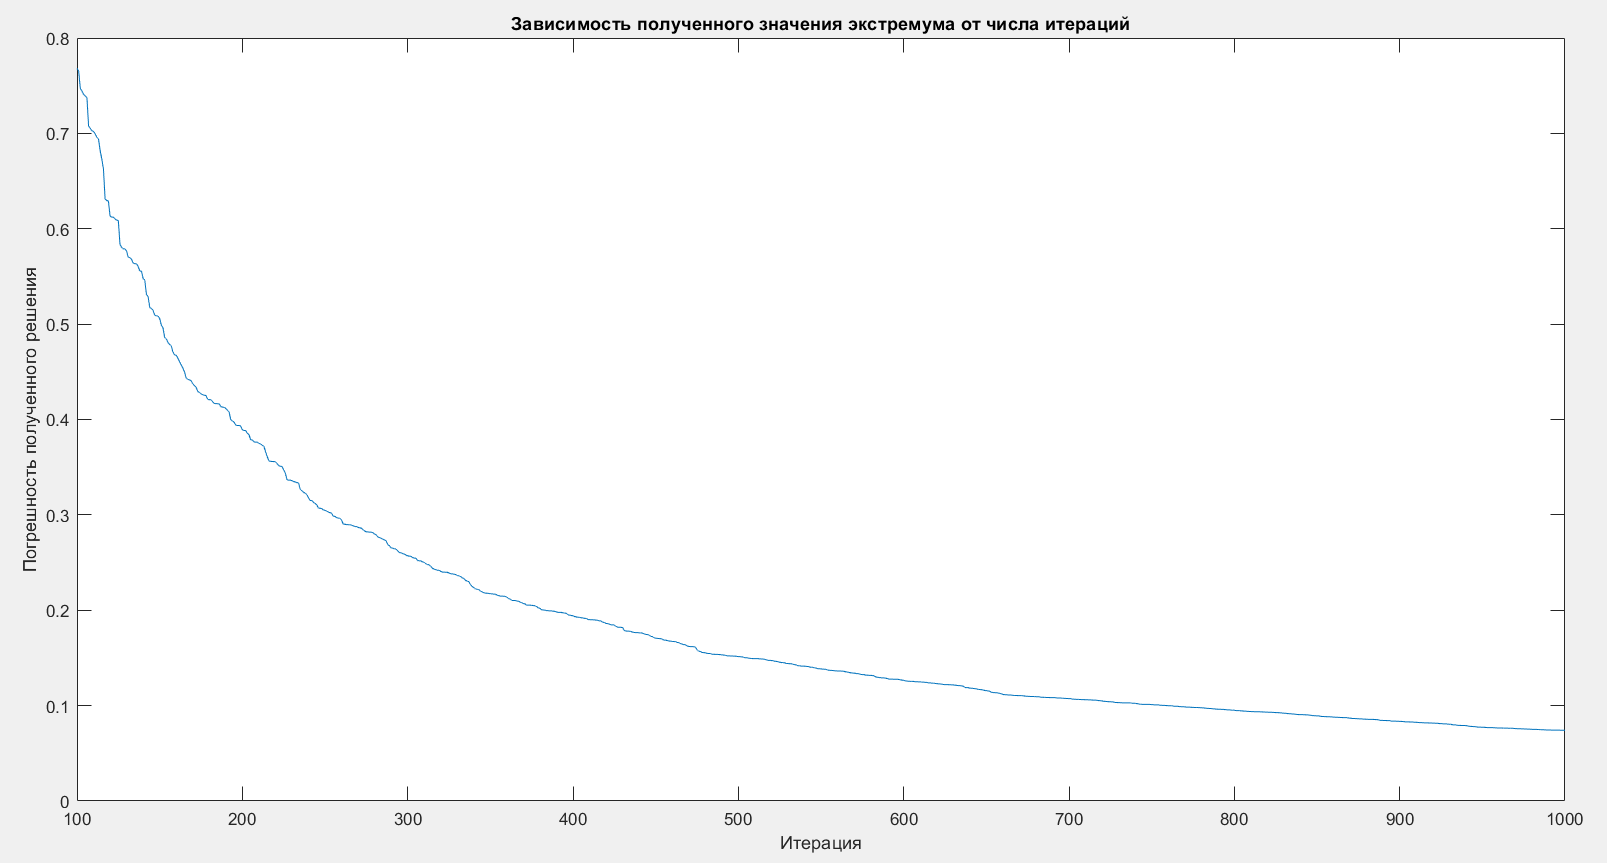
\includegraphics[width=0.75\textwidth]{mccormick_abs.png}
	\caption{Зависимость отклонения полученного экстремума от истинного значения}
\end{figure}

Из графика видно, что скорость сходимости алгоритма медленная. Чтобы достигнуть точности решения $10^{-1}$, нужно пройти 1000 итераций.



\section{Приложение}
Код программы на Python лежит в данном репозитории: \\
\url{https://github.com/PinkOink/Interval_Analysis/tree/main/lab2}{}

Реализация функции глобальной оптимизации: \\
\url{http://www.nsc.ru/interval/Programing/MCodes/globopt0.m}{}

Сайт с тестовыми функциями: \\
\url{https://en.wikipedia.org/wiki/Test_functions_for_optimization}{}


\end{document}